\documentclass[11pt, oneside]{article}   	% use "amsart" instead of "article" for AMSLaTeX format
\usepackage{geometry}                		% See geometry.pdf to learn the layout options. There are lots.
\geometry{letterpaper}                   		% ... or a4paper or a5paper or ... 
%\geometry{landscape}                		% Activate for for rotated page geometry
%\usepackage[parfill]{parskip}    		% Activate to begin paragraphs with an empty line rather than an indent
\usepackage{graphicx}				% Use pdf, png, jpg, or eps� with pdflatex; use eps in DVI mode
								% TeX will automatically convert eps --> pdf in pdflatex		
\usepackage{amssymb}
\usepackage{amsmath}
\usepackage{parskip}
\usepackage{hyperref}

\title{e as a limit}
%\author{The Author}
%\section{}
% \subsection*{R code}
\date{}							% Activate to display a given date or no date

\graphicspath{{/Users/telliott_admin/Dropbox/Tex/png/}}

% \begin{lstlisting}  \end{lstlisting}
% \begin{center} 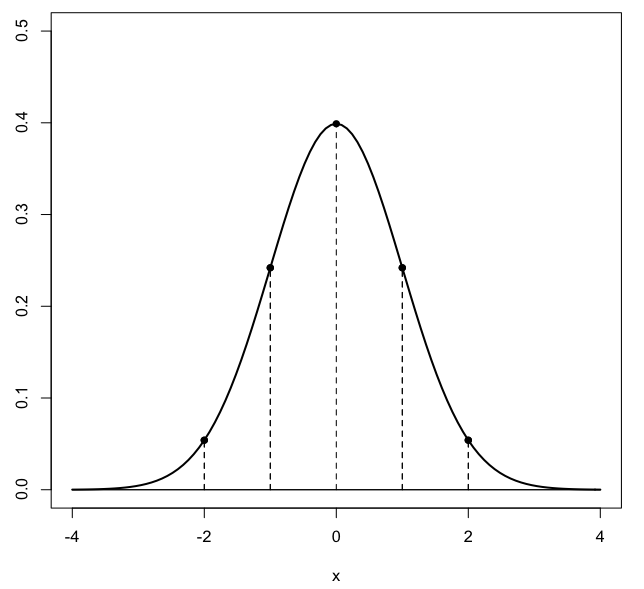
\includegraphics [scale=0.4] {gauss3.png} \end{center}
% \begin{bmatrix} a  &  b \\ c  &  d \end{bmatrix}
% \bigg |_

\begin{document}
\maketitle
\noindent
\Large

This short write-up is to demonstrate that the number $e$ is equivalent to a limit:
\[ \lim_{n \rightarrow \infty} (1 + \frac{1}{n})^n \]

I am simply following the proof as I found it online 

(here:  \url{http://aleph0.clarku.edu/~djoyce/ma122/elimit.pdf }).

So we start with a different definition of $e$ and show that it is equivalent.  We begin with this definition of the natural logarithm:
\[ \ln x = \int_1^x \frac{1}{t} \ dt \]

(We have worked through some consequences of this in a different write-up, following David Jerrison's MIT lecture.  It can be shown fairly easily that this function has all the properties of the natural logarithm).

In addition to that definition, we need two more properties, first:
\[ \ln 1 = \int_1^1 \frac{1}{t} \ dt = 0 \]

fairly obvious, since the upper and lower bounds are equal, and then second, our definition of $e$.  It is the number such that
\[ \ln e = \int_1^e \frac{1}{t} \ dt = 1 \]

So here's the proof.  Let $t$ be any number in an interval $[1, 1 + 1/n]$.  We're interested in what happens as $n$ gets large.  We have that

\[ 1 \le t \le 1 + \frac{1}{n} \]

If we invert each term, then $\le$ becomes $\ge$, but we will instead rearrange the terms:
\[ \frac{1}{1 + \frac{1}{n}} \le \frac{1}{t} \le 1 \]

The only tricky step is this one:  for each of the above, we integrate the variable $t$ between the endpoints $1$ and $1 + 1/n$, remembering that $n$ is just a number and so is $1 + 1/n$, so we have

\[ \int_1^{1 + 1/n} \frac{1}{1 + \frac{1}{n}} \ dt \le \int_1^{1 + 1/n} \frac{1}{t} \ dt \le \int_1^{1 + 1/n}  1 \ dt \]

The first integral is a constant times $t$ evaluated between $1 + 1/n$ and $1$ which is equal to the constant times $1/n$:
\[ \ [ \ \frac{1}{1 + \frac{1}{n}} \ ] \  \frac{1}{n} = \frac{1}{1 + n} \]

The second one is $\ln (1 + 1/n)$ by the definition of the logarithm, and the third is the same integral as the first but without the constant, so we have that:
\[ \frac{1}{1 + n} \le \ln (1 + \frac{1}{n} ) \le \frac{1}{n} \]

From here on, we just rearrange things a bit.  Exponentiating each term doesn't change the inequality:
\[ e^{1/1 + n} \le 1 + \frac{1}{n} \le e^{1/n}\]

The left-hand inequality can be raised to the power $(n+1)$ giving:
\[ e \le (1 + \frac{1}{n})^{n + 1} \]

and divide by $ (1 + \frac{1}{n})$
\[ \frac{e}{1 + 1/n} \le (1 + \frac{1}{n})^{n} \]

We notice that, in the limit as $n \rightarrow \infty$, this becomes 

\[ e \le  \lim_{n \rightarrow \infty} (1 + \frac{1}{n})^n \]

Similarly for the right-hand inequality, raise to the power $n$ giving:
\[ (1 + \frac{1}{n})^{n} \le e \]

and in the limit as $n \rightarrow \infty$, this becomes

\[ \lim_{n \rightarrow \infty} (1 + \frac{1}{n})^{n} \le e \]

Call the limit $L$.

The only way that $e \le L$ and $L \le e$ can both be true is if $e$ is equal to the limit in question.  This is the squeeze theorem.  Hence

\[ e = \lim_{n \rightarrow \infty} (1 + \frac{1}{n})^n \]



\end{document}  